\section{Check Patterns}

\begin{itemize}
    \item \textcolor{blue}{Separiere guten Input von schlechten Input}
    \item Jede Input-basierte Applikation braucht \textcolor{blue}{information integrity checks}. Diese Checks sollen angewendet werden, ohne dass das Programm komplizierter wird
    \item Es gibt 10 Patterns und 3 Sektionen $\rightarrow$ \textit{Meaningful Quantities, Data Manipulation} und \textit{Long Term Integrity}
\end{itemize}

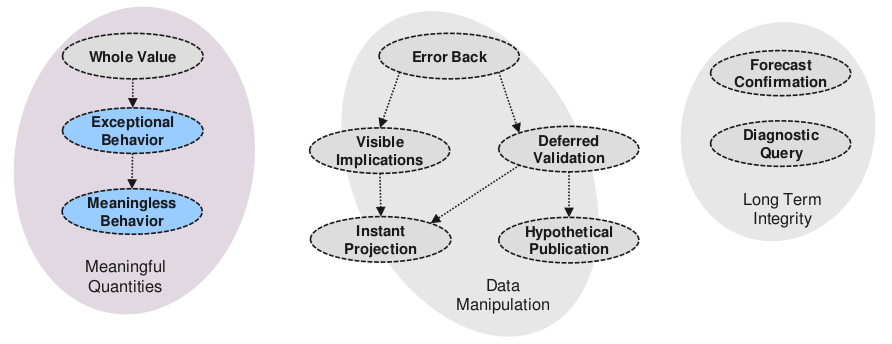
\includegraphics[width=\linewidth]{checks.png}

\subsection{Exceptional Behaviour (Meaningful Quantities)}

Fehlende oder inkorrekte Werte in einem Domain Model sind unmöglich zu verhindern. Die Domänen-Logik
sollte im Stande sein mit dieser Art von fehlenden Daten umzugehen

\subsubsection{Problem}
\begin{itemize}
    \item Missing or incorrect values in a domain model are impossible to avoid
    \item The domain logic should be able to handle this sort of missing data
    \item How can exceptional behaviour caused by invalid input be handled without throwing errors?
\end{itemize}
\subsubsection{Solution}
Verwende einen oder mehrere unterschiedliche Werte um \textit{exceptional} Umstände zu repräsentieren

\begin{itemize}
    \item \textcolor{blue}{Invalide Domainaufrufe können \textit{Exceptional Values} produzieren} \textit{Enumeration Value} als \textit{Exceptional Value} können identifizieren, was falsche gelaufen ist
    \item Domain Logik kann temporär \textit{Exceptional Values} als erlaubter Input akzeptieren
\end{itemize}
\begin{lstlisting}
// TypeScript
public div(num: number, div: number): number | CalcError {
    div === 0 ? CalcError.DivByZero : num / div;
}
\end{lstlisting}

\subsection{Meaningless Behaviour (Meaningful Quantities)}

Wegen dem Error Handling, kann die Domänen-Logik komplexer sein, als geplant. Wie kann \textit{exceptional} Verhalten wegen invalidem Input behandelt werden, ohne Errors zu werfen?

\subsubsection{Problem}
\begin{itemize}
    \item Due to error handling, domain logic may be expressed with more complexity than originally conceived
    \item How can exceptional behaviour due to invalid input be handled without throwing errors?
\end{itemize}

\subsubsection{Solution}
Schreibe Methoden \textcolor{blue}{mit minimaler Rücksicht} auf mögliche Fehler
\begin{itemize}
    \item \textcolor{blue}{Wenn ein Fehler auftritt} Erhole dich vom Fehler und mach weiter mit dem Processing. Stell sicher, dass der Error geloggt wird
    \item Wähle \textcolor{blue}{Meaningless Behaviour}, wenn eine Bedingung keine Bedeutung für einen Bereich hat
    \item Ist eine alternative für \textit{Exceptional Value} $\rightarrow$ Meaningless Behaviour biete wahrscheinlich eine tiefer error-information Granularität
\end{itemize}
\begin{lstlisting}
// TypeScript
public div(num: number, div: number): number {
    return num / div; // Infinity (Java NaN) if div == 0
}
\end{lstlisting}
